\documentclass[%
bachelor,    % тип документа
natbib,      % использовать пакет natbib для "сжатия" цитирований
subf,        % использовать пакет subcaption для вложенной нумерации рисунков
href,        % использовать пакет hyperref для создания гиперссылок
colorlinks,  % цветные гиперссылки
%fixint,     % включить прямые знаки интегралов
]{disser}

\usepackage[
a4paper, mag=1000,
left=2.5cm, right=1cm, top=2cm, bottom=2cm, headsep=0.7cm, footskip=1cm
]{geometry}

\usepackage[intlimits]{amsmath}
\usepackage{amssymb,amsfonts}

\usepackage[T2A]{fontenc}
\usepackage[utf8]{inputenc}
\usepackage[english,russian]{babel}
\ifpdf\usepackage{epstopdf}\fi
\usepackage[autostyle]{csquotes}

% Шрифт Times в тексте как основной
%\usepackage{tempora}
\usepackage{setspace}
% альтернативный пакет из дистрибутива TeX Live
%\usepackage{cyrtimes}

% Шрифт Times в формулах как основной
%\usepackage[varg,cmbraces,cmintegrals]{newtxmath}
% альтернативный пакет
%\usepackage[subscriptcorrection,nofontinfo]{mtpro2}

% Плавающие рисунки "в оборку".
\usepackage{wrapfig}

% Номера страниц снизу и по центру
%\pagestyle{footcenter}
%\chapterpagestyle{footcenter}

% Точка с запятой в качестве разделителя между номерами цитирований
%\setcitestyle{semicolon}

% Использовать полужирное начертание для векторов
\let\vec=\mathbf
%______________________________-
\usepackage{lipsum}

%\usepackage{titlesec}
%\usepackage{spacing}
%\titleformat{\section}[block]{\color{blue}\Large\bfseries\filcenter}{}{1em}{}
% Номера страниц снизу и по центру
\pagestyle{footcenter}
\chapterpagestyle{footcenter}

% Точка с запятой в качестве разделителя между номерами цитирований
%\setcitestyle{semicolon}



% Переопределение стандартных заголовков
%\def\contentsname{Содержание}
%\def\conclusionname{Выводы}
%\def\bibname{Литература}

\usepackage{geometry} % пакет для установки полей
\geometry{top=1.5cm} % отступ сверху
\geometry{bottom=2cm} % отступ снизу
\geometry{left=3cm} % отступ справа
\geometry{right=1.5cm} % отступ слева
\newcommand{\sectionbreak}{\clearpage}
\newcommand*{\No}{\textnumero}
\renewcommand{\Re}{\mathrm{Re}}
\renewcommand{\Im}{\mathrm{Im}}

\newcommand{\const}{\mathrm{const}}
\newcommand{\arccosh}{\mathrm{arccosh}}

\newcommand{\vF}{\mathbf{F}}
\newcommand{\ve}{\mathbf{e}}
\newcommand{\vk}{\mathbf{k}}
\newcommand{\vq}{\mathbf{q}}
\newcommand{\vp}{\mathbf{p}}
\newcommand{\va}{\mathbf{a}}
\newcommand{\vP}{\mathbf{P}}
\newcommand{\vK}{\mathbf{K}}
\newcommand{\vQ}{\mathbf{Q}}
\newcommand{\vA}{\mathbf{A}}
\newcommand{\vr}{\mathbf{r}}
\newcommand{\vR}{\mathbf{R}}

\newcommand{\vRR}{\boldsymbol{\mathcal{R}}}
\newcommand{\veps}{\boldsymbol{\varepsilon}}

\newcommand{\cA}{\mathcal{A}}
\newcommand{\cR}{\mathcal{R}}
\newcommand{\cM}{\mathcal{M}}
\newcommand{\cE}{\mathcal{E}}
\newcommand{\cJ}{\mathcal{J}}
\newcommand{\cT}{\mathcal{T}}
\newcommand{\cD}{\mathcal{D}}


%______________________________-
% Включать подсекции в оглавление
\setcounter{tocdepth}{2}

\graphicspath{{fig/}}

\begin{document}
\section*{\centering Введение}
\addcontentsline{toc}{section}{Введение}

Вопрос о том, из чего сделан материальный мир и откуда все это произошло, интересовал людей со времен античности. Левкипп (около 430 г. до н.э.) и Демокрит
(около 420 г. до н.э.) первыми предложили атомную теорию, в которой вся материя состоит из
неделимых частиц. В средние века, различные исследователи, известные как алхимики, добились прогресса
в разработке экспериментальных методов исследования составляющих компонентов вещества. Однако,
их исследования в основном состояли из тщетных попыток превратить обычные металлы
(например, свинца) в благородные металлы (такие как золото), и не было достигнуто никакого прогресса в
развитии теории о том, как может произойти такое преобразование. Только в конце 20-го века современные алхимики, обычно
известные как ядерные физики, добились успеха в превращении висмута в золото
(в небольших количествах и по коммерчески неосуществимым расходам). Дорога, ведущая к этому знаменательному достижению, включала работы химиков (Бойл, 1661, де Лавуазье, 1789), современную атомной теории (Dalton, 1808, Avogadro, 1811, Thomson, 1897) и достижения в ядерной физике (Резерфорд, 1911; Чадвик, 1932; Ферми, 1934; Юкава, 1935), которые обеспечили нам хорошее понимание строительных блоков, из которых состоит материя.

Хорошее понимание того, что составляет материю, является необходимым первым шагом в развитии теорию о том, как эта материя была создана.  Alpher et al. (1948) выдвинул теорию, что все элементы были синтезированы во время Большого взрыва. Однако, когда более точнее сечение захвата нейтронов для ядер малой массы (A < 20) стало доступным, также стало ясно, что нуклеосинтез во время ранней расширяющейся вселенной не способен преодолеть A = 8 (например, Alpher and Herman, 1950; Shaviv, 2012). Это легло в основу работы Burbidge et al. (1957), который предложил, что лишь самые легкие элементы (в основном водород и гелий) возникли во время Большого взрыва, а более тяжелые элементы синтезируются в звездах. Хотя эта теория со временем была уточнена, оригинальная идея Бербиджа и др. (1957) выдержал испытание временем. Таково нынешнее понимание того, что различные ядерные процессы действительно ответственны за синтез всех элементов, более тяжелых, чем водород и гелий.

В данной работе я исследую процесс захвата быстрых нейтронов (r-процесс), который является одним из ядерных процессов, предположенных Burbidge et al. (1957) в результате которого возникают элементы тяжелее железа. Мое внимание сосредоточено на вычислении нуклеосинтеза r-процесса при слияним звезд при помощи нового инструмента для расчета ядерных реакций, SkyNey, который я разработал. В оставшейся части этого введения я кратко опишу текущее представление о происхождении элементов, сущность r-процесса, условия его возникновения и ожидаемые наблюдательные сигнатуры. В главе II я представляю физику, которая реализована в SkyNet для эволюции тысяч видов ядер под влиянием десятков тысяч ядерных реакций Я использую SkyNet в главе III, чтобы систематически исследовать r-процесс и его возможные оптические аналоги для различные параметров. В главе IV обсуждается нуклеосинтез r-процесса при слияниях черных дыр и нейтронных звезд (BHNS), а в главе V я рассматриваю rprocess
в оттоке диска (in the disk outflow following) после слияния нейтронных звезд. В главе VI я кратко подведу итог другой работы, которую я проделал во время моей докторской диссертации, которая не является непосредственно частью этой работы. Наконец, я предоставляю резюме и дальнейшие перспективы в главе VII.

\subsection{Распространенность в солнечной системе}
Стоит проверить теории и модели, которые предсказывают как создаются элементы и в каких отношениях, подробный перечень этих элементов и их относительная распространенность в данном участки вселенной. Крайне сложно получить образцы материи из мест, отличных от земной коры. Миссии Аполлона и Луны принесли образцы с луны, а позже такие космические аппараты, как Звездная пыль, Бытие и Hayabusa успешно доставили образцы из близлежащих астероидов и космической пыли на Землю. Однако подавляющее большинство внеземных материалов, доступных для химических анализов происходит от метеоритов, которые падают на поверхность Земли. Поэтому, чтобы определить состав звезд и других астрофизических объектов, мы ограничимся изучением линиями поглощения и излучения, формирующими эти объекты, а также распространенность элементарных частиц (например, Shaviv, 2012). Линии поглощения в солнечном спектре были впервые обнаружены в начале XIX век (Wollaston, 1802; Fraunhofer, 1817). Тем не менее, применение им нашли только 100 лет спустя, после развития квантовой механики, которая утверждает, что линии поглощения могут использоваться для количественного определения распространенности различных элементов на солнце. Пионерская работа была проведена Пейном (1925) в ее основной научной диссертации и Расселом (1934). Важная работа Суссе и Юри (1956) была одной из первых принимающих во внимание изотопные измерения распространенности из метеоритов. С этого момента был достигнут большой прогресс в измерении распространенности элементов и изотопов в нашей солнечной системе (например, Cameron, 1973; Anders and Grevesse, 1989; Grevesse and Sauval, 1998; Lodders, 2003).

\begin{figure}[h]
	\center{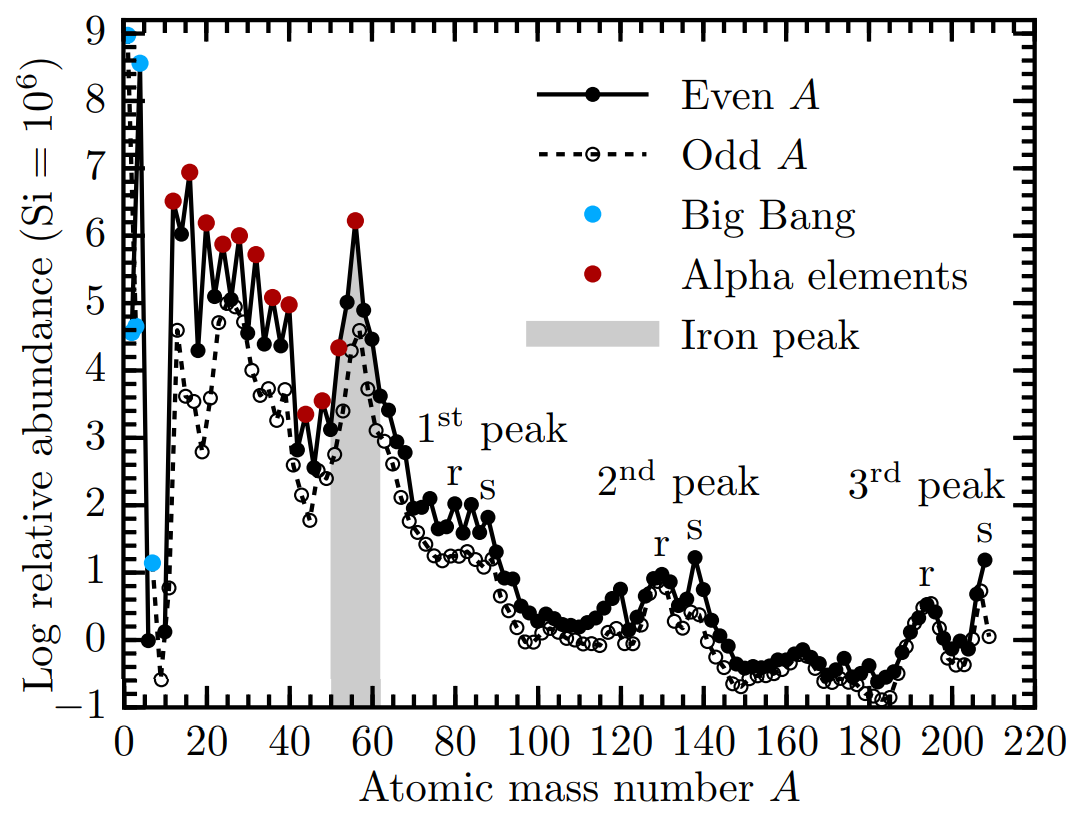
\includegraphics[width=0.7\linewidth]{1}}
	\caption{Наблюдаемая распространенность в нашей солнечной системе в зависимости от массового числа А. Самые легкие элементы были созданы в «Большом взрыве». Слияние в звездах преимущественно создает альфа-элементы. Пик железа выполнен в коллапсе ядра и типе Ia сверхновых. Элементы за железным пиком синтезируются медленными (s) и быстрыми (r) процессами захвата нейтронов. Эти процессы производят три пары пиков (см. раздел 1.3). Данные о изобилии от Lodders (2003).}
	\label{ris:1}
\end{figure}

На рис. \ref{ris:1} показаны наблюдаемые распространенности в нашей солнечной системе в зависимости от массового числа А (данные от Lodders 2003). Нуклиды с четным массовым числом как правило более многочисленными, чем нуклиды с нечетным массовым числом, поскольку даже массовые нуклиды более связаны. (!!!!!!even mass nuclides are more bound) Из-за спинового спаривания нуклонов нуклид с четным число нейтронов и протонов (следовательно, четное A) является более связанным, чем нуклид с нечетным числом нейтронов или протонов (следовательно, нечетное А, см., например, Weizsäcker, 1935; Майерс и Свитецки, 1966; Möller et al., 1995). Нуклиды с нечетное число и нейтронов и протонов (отсюда и четное A), имеют еще более слабую связь поскольку ни все нейтроны, ни все протоны не могут быть спин-парными. Поэтому неудивительно, что существует только несколько нечетных-нечетных нуклидов, которые являются стабильными или долгоживущими: 2H, 6Li, 10B и 14N стабильны, а 40K, 50V, 138La и 176Lu являются только нечетные-нечетные нуклиды с периодом полураспада не менее 1 Гр(!!!!!Gyr). Существует ряд различных процессов нуклеосинтеза, которые доминируют в различных диапазонах масс. Очень легкие нуклиды (A <8) были получены сразу после Большого взрыва. Некоторые $^4He$, а также большинство нуклидов в диапазоне 12 $<=$ A $<=$ 56 являются результатом гидростатического ядерного горения в звездах, значительная часть пика железа (50 .A .62) производится материалом, поступающим в (!!!!!nuclear statistical equilibrium) ядерную статистическую (NSE), а затем охлаждающимся (например, во время сверхновой звезды Ia или взрывчатое сильное сжигание в ядрах с коллапсом сверхновых (explosive silicon burning in core-collapse supernovae) (CCSNe)) и, наконец, почти все нуклиды, более тяжелые, чем железо, образуются путем захвата нейтронов на более легкие семенные ядра (!!!!!onto lighter seed nuclei) (например, Burbidge et al., 1957). Мы рассмотрим эти процессы далее.

\subsection{Нуклеосинтез Большого Взрыва}
\begin{figure}[h]
	\center{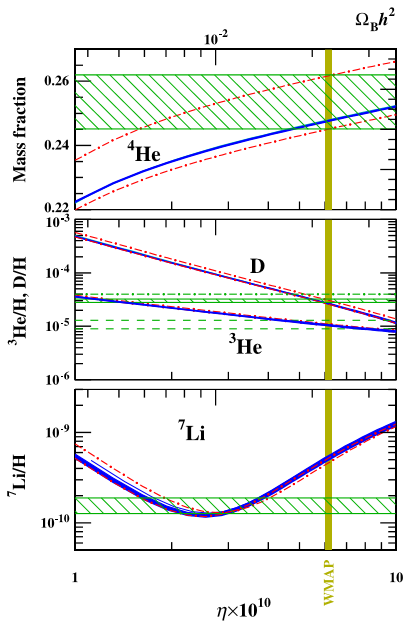
\includegraphics[width=0.7\linewidth]{2}}
	\caption{Вычисленная распространенность 4He, D, 3He и 7Li (синие линии) в зависимости от отношения барион-фотон $\eta$. Зеленые области - наблюдаемые концентрации, а желтая вертикальная полоса - наблюдаемое значение $\eta$. Вычисленные количества 4He, D и 3He согласуются с наблюдениями, но прогнозируется избыток 7Li в 4-5 $\sigma$. Это известная «литиевая проблема». Рисунок 1 из Cocetal. (2013)}
	\label{ris:2}
\end{figure}
Нуклеосинтез Большого Взрыва (BBN) создал в основном водород (~ 75$\%$ по массе) и гелий (~ 25$\%$ по массе) в промежутке от первых десяти секунд до минут после Большого взрыва, а также некоторое количества (!!!!trace - следовое) дейтерия, 3He и 7Li (см. Tytler et al., 2000 и ссылки в нем). 13,8 Gyr позже химический состав Вселенной оставался около 75$\%$ H и 25$\%$ He, потому что создание более тяжелых элементов требует экстремальных физических условий. Интересно, что BBN является проблемой для моделирования, потому что он включает лишь несколько нуклидов, в настоящее время существуют большие расхождения между результатами моделирование BBN и наблюдениями. Прогнозируемый дейтерий и распространенность 4He хорошо согласуется с наблюдениями, но модели BBN предсказывают большую распространенность 7Li на 4-5 $\sigma$ по сравнению с наблюдениями, см. рис. \ref{ris:2}, которая изображена на рисунке 1 от Coc et al. (2013). Это расхождение не до конца понятно и называется «литиевой проблемой». Предлагаемые причины этого включают систематические ошибки в наблюдениях численности 7Li, неизвестные или плохо измеренные ядерные свойства 7Be и даже неизвестные физические процессы, протекающий за гранью Стандартной модели.
См., например, поля (2011) и ссылки в них.
\subsection{Ядерное горение в звездах малой массы}
\begin{figure}[h]
	\center{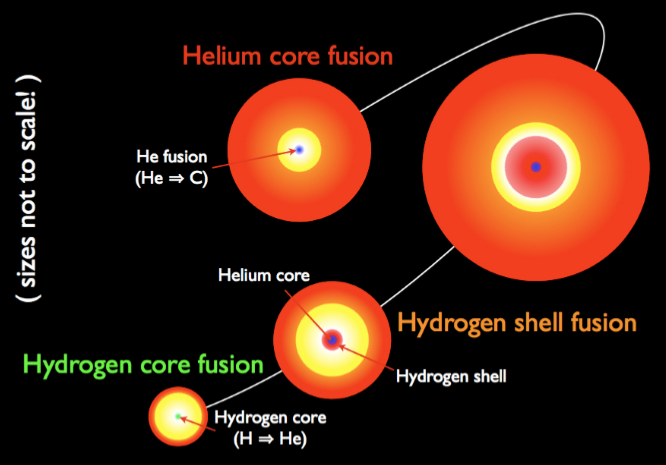
\includegraphics[width=0.7\linewidth]{3}}
	\caption{Изображение ранних этапов эволюции звезд. Звезда начинается со слияния	водорода с гелием. Когда водород в активной зоне истощен, ядро сжимается, что повышает температуру и запускает водородное слияние (!!!fusion) в оболочке вокруг гелиевого ядра. Это расширяет атмосферу звезды и превращает ее в		красного гиганта. После сжигания водородного топлива ядро снова сжимается под 	действием силы тяжести, которая увеличивает температуру до той отметки, при которой синтез начинался. Рисунок из $https://www.nasa.gov/mission\_pages/$}
	\label{ris:3}
\end{figure}

Главное препятствие объединения гелия и водорода в тяжелые элементы - это сильное Кулоновское отталкивание между нуклидами, которые все положительно заряжены. Более того, стандартный способ плавления (!!!!fuse может быть синтез) водороде это p-p цепь, включающая слабую реакцию p + p $\rightarrow$ d + e + + $\nu$e, которая имеет чрезвычайно малое сечение (!!!!!cross section) (Rolfs and Rodney, 1988). Поэтому чрезвычайно высокие температуры ($\&$ 10 MK) являются необходимо для сжигания водорода в гелий и гелий в более тяжелые элементы. Такие условия достигаются внутри звезд, где происходит ядерный синтез (например, Бете 1939), высвобождая энергию ядерной связи в виде тепла, удерживающую звезду от разрушения и заставляя ее сиять.
На рис. \ref{ris:3} изображены ранние стадии эволюции звезд. По определению, каждая звезда, по крайней мере, синтезирует водород в гелий внутри ядра, и звезды проводят большую часть своей жизни в этой фаза горения водорода. Как только запас водорода в ядре исчерпан, температура становится недостаточно высокой для сжигания гелия, поэтому ядро сжимается, потому что источник тепла от сжигания водорода уменьшается. Далее (!!!As the core contracts), он нагревается, и температура становится достаточно высокой для горения водорода в оболочке вокруг гелиевого ядра. В этот момент атмосфера звезды быстро расширяется, и звезда входит в фазу красного гиганта. Когда водород в оболочке исчерпан и, если звезда достигла определенных массы ($\&$ 0,5 М, например, Рольфс и Родни, 1988), ядро снова сжимается, то есть увеличивается температура и становится возможен тройной-альфа процесс, который синтезирует (!!!преобразует) три частицы 4He в 12C. Некоторые гелиевые сплавы также могут быть преобразованы с вновь созданным 12C, чтобы создать 16O, и, в принципе, он также может пойти дальше, производя 20Ne, 24Mg, 28Si и т. д., которые называются альфа-элементами, потому что они являются определенным количество альфа-нуклидов, слитых вместе. Однако на практике реакция 16O + 4He $\rightarrow$ 20Ne является медленной, и поэтому сжигание гелия в основном производит 12C и 16O (см. Rolfs and Rodney, 1988; Hansen et al., 2004). Когда гелий истощается, температура ядра снова повышается за счет сжатия. Наибольшая температура, достигаемая в звезде, зависит от ее начальной массы. Если начальная масса выше ~ 8 М, то углерод и кислород могут быть сожжены, в противном случае звезда заканчивает свою жизнь как углерод-кислородный белый карлик (например, Rolfs and Rodney, 1988; Hansen et al., 2004). Если масса звезда представляет собой лишь несколько солнечных масс выше 8 М, она может быть способна сжигать углерод, а затем стать белым карликом кислорода-неонового цвета.
\subsection{Ядерное горение в тяжелых звездах}

\begin{figure}[h]
	\center{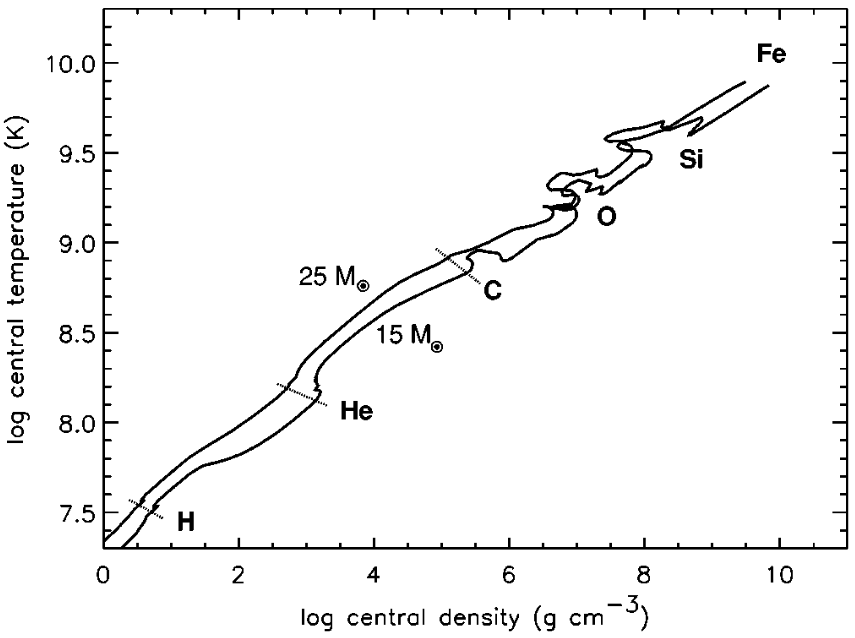
\includegraphics[width=0.7\linewidth]{4}}
	\caption{Центральная плотность и температура 15M, а также 25M звездных моделей. По мере развития звезды центральная плотность и температура возрастают, последовательно воспламеняются водород, гелий, углерод, кислород и сгорает кремний. Рисунок 1 из Woosley et al. (2002) © 2002 Американское физическое общество}
	\label{ris:4}
\end{figure}

Звезды с начальной массой более 8 М проходят через несколько стадий горения. После каждого этапа, ядро сжимается под действием сил тяжести, поскольку ядерное топливо на этой стадии был исчерпано и, следовательно, источник ядерного тепла потерян. Поскольку ядро сжимаются, они нагревается, что позволяет начать следующую стадию горения, если температура будет достаточно высока. Это показано на рис. 1.4 (рис. 1 из Woosley et al., 2002), который показывает центральную плотность и температуру двухзвездной модели и областей, в которых происходят различные стадии горения. В фазе сжигания углерода существуют ряд различных реакции 12C + 12C, но чаще всего наблюдается 20Ne + 4He и 23Na + p. Свободный протон может захватывать другие существующие нуклиды для создания не-альфа-элементов, а также 23Na, являющийся не-альфа-элементом, который могут быть преобразован в другие не-альфа-элементы. Гелий, полученный из сгорания углерода также сжигается как 12C + 4He $\rightarrow$ 16O или 16O + 4He $\rightarrow$ 20Ne. Когда углерод истощается, ядро сжимается до тех пор, пока очень энергичные фотоны (!!!very energetic photons) формирующие хвост Распределения Планка не смогут фото-синтезировать 20Ne, что приводит к образованию свободных альфа-частиц, которые могут захватывать недиссоциированные 20Ne, чтобы сформировать около 24Mg. Реакция с низшим кулоновским барьером теперь 16O + 16O, что в основном приводит к 28Si + 4Не и 31P + p (см. Rolfs and Rodney, 1988). Освобожденные альфа-частицы захватываются на 24Mg и 28Si, чтобы сформировать 28Si и 32S.
В конце сжигания кислорода звездное ядро состоит в основном из 28Si, 32S и небольшого количества других нуклидов. Это является предпосылкой для окончательной фазы горения: сжигание силикона. Перед тем, как температура, требуемая для 28Si + 28Si достигается, кремниевые нуклиды разрушаются фото-диссоциацией, что снова создает источник для свободных альфа-частиц. Эти альфа-частицы захватываются последовательно, начиная с 28Si для создания 32S, 36Ar, 40Ca, 44Ti, 48Cr, 52Fe и 56Ni, что называется альфа процессом или альфа-лестницой, которая встречается на временной шкале (см. Рольфс и Родни, 1988; Hansen et al., 2004). Поскольку температура во время сжигания кремния настолько высока ($\&$ 3,5 ГК), нуклиды, более тяжелые, чем кремний, также могут быть фото-диссоциированными (!!!photodissociated). Результатом являются такие реакции, как 28Si + 4He $\rightarrow$ 32S, которые находятся в равновесии с их обратными реакции. Таким образом, существует группа нуклидов, а именно нуклидов с 28 $<=$ A $<=$ 62, свободные альфа-частицы, нейтроны и протоны, находящихся в равновесии друг с другом. Это состояние называется квазиравновесным (QSE) и отличается от NSE (см. Следующий раздел) тем, что не все нуклиды находятся в равновесии друг с другом. В частности, 12C, 16O, 20Ne, и 24Mg не являются частью группы QSE, описанной выше (например, Bodansky et al.,1968; Woosley et al., 1973).
Однако сжигание сита может производить только нуклиды вплоть до атомного массового числа от А = 56, так как энергия связи на нуклон (протоны и нейтроны) достигает максимум при этой массе. Поэтому более тяжелые нуклиды более слабо связаны (Rolfs и Rodney, 1988), что означает, что нужно добавить энергию, чтобы обеспечить слияние за пределами A = 56. Другими словами, как только все значимые элементы в ядре массивной звезды сожжены до 56Ni (Ничего не понял), сердцевина звезды будет состоять из ядерной пыли, которая не может гореть, а звезда теряет свой основной источник тепла. Ядро остается поддерживаемым от коллапса давлением вырождения электрона, но как только масса ядра


\bibliographystyle{utf8gost705u}  %% стилевой файл для оформления по ГОСТу
\end{document} 